% Author: Izaak Neutelings (September 2020)
\documentclass[border=3pt,tikz]{standalone}
\usepackage{amsmath}
\usepackage{tikz}
\usepackage{physics}
\usepackage{siunitx}
\usepackage[outline]{contour} % glow around text
\usetikzlibrary{angles,quotes} % for pic
\contourlength{1.3pt}

\tikzset{>=latex} % for LaTeX arrow head
\usepackage{xcolor}
\colorlet{veccol}{green!70!black}
\colorlet{vcol}{green!70!black}
\colorlet{xcol}{blue!85!black}
\colorlet{projcol}{xcol!60}
\colorlet{unitcol}{xcol!60!black!85}
\colorlet{unitcol2}{vcol!60!black!85}
\colorlet{myblue}{blue!70!black}
\colorlet{myred}{red!70!black}
\tikzstyle{vector}=[->,very thick,xcol]
\tikzstyle{mydashed}=[dash pattern=on 2pt off 2pt]
\def\tick#1#2{\draw[thick] (#1) ++ (#2:0.1) --++ (#2-180:0.2)} %0.03*\xmax


\begin{document}


% CIRCLE polar coordinates + vector
\def\xmax{2.0}
\def\ul{0.6}
\def\R{1.7}
\begin{tikzpicture}
  \def\ang{43}
  \coordinate (O) at (0,0);
  \coordinate (X) at (\xmax,0);
  \coordinate (R) at (\ang:\R);
  \draw[->,line width=0.9] (-\xmax,0) -- (1.08*\xmax,0) node[right] {$x$};
  \draw[->,line width=0.9] (0,-\xmax) -- (0,1.08*\xmax) node[left] {$y$};
  \node[fill=black,circle,inner sep=0.9] (R') at (R) {};
  \node[above right] at (R) {$(x,y)=(r;\theta)$};
  \draw[vector] (O) -- (R') node[midway,left=5,above right=0] {$\vb{r}$};
  \draw pic[->,"$\theta$",draw=black,angle radius=21,angle eccentricity=1.2] {angle=X--O--R};
  \draw (O) circle (\R);
  \draw[dashed] (R) -- ({\R*cos(\ang)},0);
  \draw[dashed] (R) -- (0,{\R*sin(\ang)});
  \draw[vector,<->,unitcol]
    (\ul,0) node[scale=1,left=4,below right=-3] {$\vu{x}$} -- (O) --
    (0,\ul) node[scale=1,below=4,above left=-3] {$\vu{y}$};
  \draw[vector,<->,unitcol2] %,line cap=round
    (\ang:\ul) node[scale=1,left=0,above left=-3] {$\vu{r}$} -- (O) --
    (\ang+90:\ul) node[scale=1,left=-3] {$\vu*{\theta}$};
  \draw[vector,->,unitcol2,line cap=round]
    (R) --++ (\ang+90:\ul) node[scale=1,above left=-3] {$\vu*{\theta}$};
  %\draw[thick] ({\R*cos(\ang)},0.1) --++ (0,-0.2) node[scale=0.9,below=-1] {$r$};
  %\draw[thick] (0.1,{\R*sin(\ang)}) --++ (0,-0.2) node[scale=0.9,left=-1] {$r$};
  %\draw[thick] (\R,0.1) --++ (0,-0.2) node[scale=0.9,below=-1] {\contour{white}{$r$}};
  %\draw[thick] (0.1,\R) --++ (-0.2,0) node[scale=0.9,left=-1] {\contour{white}{$r$}};
  \tick{\R,0}{90} node[below=-1] {\contour{white}{$r$}};
  \tick{0,\R}{ 0} node[left=-1] {\contour{white}{$r$}};
\end{tikzpicture}


% CIRCLE arc segment
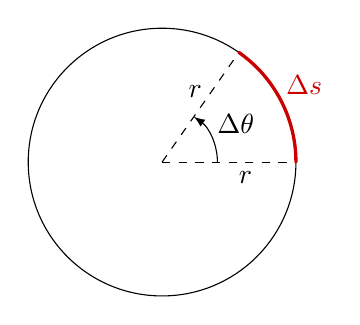
\begin{tikzpicture}
  \def\R{1.7}
  \def\ang{55}
  \coordinate (O) at (0,0);
  \coordinate (X) at (\R,0);
  \coordinate (R) at (\ang:\R);
  %\draw[vector] (O) -- (R) node[midway,right=4,above left=0] {$\vb{r}$};
  \draw[dashed] (O) -- (X) node[midway,below right=0] {$r$};
  \draw[dashed] (O) -- (R) node[midway,right=4,above left=0] {$r$};
  \draw pic[->,"$\Delta\theta$",draw=black,angle radius=20,angle eccentricity=1.5] {angle=X--O--R};
  \draw (O) circle (\R);
  \draw[red!80!black,very thick,line cap=round] (X) arc (0:\ang:\R) node[midway,above right=-2] {$\Delta s$};
  %\draw[dashed] (R) -- ({\R*cos(\ang)},0);
  %\draw[dashed] (R) -- (0,{\R*sin(\ang)});
\end{tikzpicture}


% CIRCLE unit circle
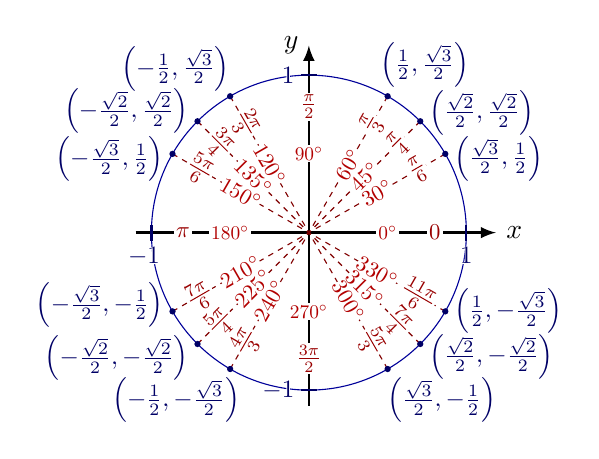
\begin{tikzpicture}
  \def\xmax{2.2}
  \def\ul{0.6}
  \def\R{2.0}
  \def\ang{43}
  \coordinate (O) at (0,0);
  \coordinate (X) at (\xmax,0);
  \coordinate (R) at (\ang:\R);
  
  % AXIS
  \draw[->,line width=0.9] (-\xmax,0) -- (1.08*\xmax,0) node[right] {$x$};
  \draw[->,line width=0.9] (0,-\xmax) -- (0,1.08*\xmax) node[left] {$y$};
  %\node[fill=black,circle,inner sep=0.9] (R') at (R) {};
  %\node[above right] at (R) {$(x,y)=(r;\theta)$};
  \draw[blue!60!black] (O) circle (\R);
  
  \def\tick#1#2{\draw[blue!40!black,thick] (#1) ++ (#2:0.1) --++ (#2-180:0.2)} %0.03*\xmax
  \def\axis#1#2{
    \node[red!70!black,fill=white,inner sep=1,scale=0.70] at (#1:0.5*\R) {\SI{#1}{\degree}};
    \node[red!60!black,fill=white,inner sep=1,scale=0.82] at (#1:0.8*\R) {#2};
  }
  \def\line#1#2#3#4#5{
    \draw[mydashed,red!50!black] (#1:\R) -- (O);
    \node[red!70!black,fill=white,inner sep=0,rotate=#2,scale=0.8] at (#1:0.5*\R) {\SI{#1}{\degree}};
    \node[red!60!black,fill=white,inner sep=0,rotate=#2,scale=0.9] at (#1:0.8*\R) {#4};
    \node[blue!40!black,anchor=#3,scale=0.9] at (#1:\R) {#5}; %#1-180 %sign(#2)*(90-abs(#2)) %40
    \fill[blue!40!black] (#1:\R) circle (0.04);
  }
  
  \tick{ \R,0}{90} node[scale=0.9,below=-1]        {\contour{white}{$1$}};
  \tick{0, \R}{ 0} node[scale=0.9,left=-1]         {\contour{white}{$1$}};
  \tick{-\R,0}{90} node[scale=0.9,left=3,below=-1] {\contour{white}{$-1$}};
  \tick{0,-\R}{ 0} node[scale=0.9,left=-1]         {\contour{white}{$-1$}};
  \axis{  0}{$0$}
  \line{ 30}{ 30}{175}{$\frac{  \pi}{6}$}{$\left( \frac{\sqrt{3}}{2}, \frac{1}{2}       \right)$}
  \line{ 45}{ 45}{188}{$\frac{  \pi}{4}$}{$\left( \frac{\sqrt{2}}{2}, \frac{\sqrt{2}}{2}\right)$}
  \line{ 60}{ 60}{220}{$\frac{  \pi}{3}$}{$\left( \frac{1}{2},        \frac{\sqrt{3}}{2}\right)$}
  \axis{ 90}{$\frac{\pi}{2}$}
  \line{120}{-60}{-25}{$\frac{ 2\pi}{3}$}{$\left(-\frac{1}{2},        \frac{\sqrt{3}}{2}\right)\!\!$} %\vspace{-4mm}
  \line{135}{-45}{ -8}{$\frac{ 3\pi}{4}$}{$\left(-\frac{\sqrt{2}}{2}, \frac{\sqrt{2}}{2}\right)$}
  \line{150}{-30}{  5}{$\frac{ 5\pi}{6}$}{$\left(-\frac{\sqrt{3}}{2}, \frac{1}{2}       \right)$}
  \axis{180}{$\pi$}
  \line{210}{ 30}{ -5}{$\frac{ 7\pi}{6}$}{$\left(-\frac{\sqrt{3}}{2},-\frac{1}{2}       \right)$}
  \line{225}{ 45}{ 10}{$\frac{ 5\pi}{4}$}{$\left(-\frac{\sqrt{2}}{2},-\frac{\sqrt{2}}{2}\right)$}
  \line{240}{ 60}{ 30}{$\frac{ 4\pi}{3}$}{$\left(-\frac{1}{2},       -\frac{\sqrt{3}}{2}\right)$}
  \axis{270}{$\frac{3\pi}{2}$}
  \line{330}{-30}{180}{$\frac{11\pi}{6}$}{$\left( \frac{1}{2},       -\frac{\sqrt{3}}{2}\right)$}
  \line{315}{-45}{170}{$\frac{ 7\pi}{4}$}{$\left( \frac{\sqrt{2}}{2},-\frac{\sqrt{2}}{2}\right)$}
  \line{300}{-60}{150}{$\frac{ 5\pi}{3}$}{$\left( \frac{\sqrt{3}}{2},-\frac{1}{2}       \right)$}
  
  
  
\end{tikzpicture}


\end{document}